%!TEX root = ../../thesis.tex
%\subsection{Preliminaries on Lie groups}
Throughout this work, we will explore Lie group theory. We introduce the following notations: the Lie group of rigid-body transformation on $\R^3$ is denoted by $\SE{3}$, whereas the group of homogeneous rotation is denoted by $\SO{3}$. The tangent space at the identity of the group is called the Lie algebra, and it can be used to describe the evolution of the Lie group. The Lie algebra of $\SE{3}$ and $\SO{3}$ are denoted by $\seg{3}$ and $\sog{3}$, respectively. Lastly, the cross operator (\ie, "$\times$") and hat operator (\ie, "$\wedge$") are used to transform a column vector of $\R^3$ or $\R^6$ into an element of the Lie algebra $\sog{3}$ or $\seg{3}$, respectively. A comprehensive introduction is given in Appendix \ref{app:C3:liegroup} based on the work of Bullo (1995, \cite{Bullo1995}). 
%
%
% \begin{figure}[!t]
%   \vspace{-0.6mm}
%   \centering
%   \ifx\printFigures\undefined
%   \else
%   \includegraphics[width = 0.99\textwidth]{fig_C3_schematic.pdf}
%   \fi
%   \caption{Schematic representation of the Piece-wise Constant Curvature model (PCC) for general soft robotic system, given by a parameterized curve $^0 \gammaB: \Xs \times \Ts \to \R^3$ and orientation matrix $^0 \PhiB: \Xs \times \Ts \to \SO{3}$. The frame $\{\sigma\}$ is rigidly attached to $^0 \gammaB$ such that variation of $\sigma$ give insight into the differential geometry of the curve.}
%   \label{fig:C2:configuration}
% \end{figure}
% %
\begin{figure}[!t]
  \vspace{-0.6mm}
  \centering
 \includegraphics[width = 0.99\textwidth]{3_chapters/3_chapter/img/fig_C3_schematic.pdf}
  \caption{Schematic representation of the continuously variable Cosserat beam model for a general class of soft manipulators, given by a backbone $^0 \gammaB: \Xs \times \Ts \to \R^3$ and orientation matrix $^0 \PhiB: \Xs \times \Ts \to \SO{3}$. This forms a parameterized curve $\gB = (^0 \PhiB,\,^0\gammaB) \in \SE{3}$. The representation of the soft robot is inspired by the octopus' tentacle whose the muscle forces are modelled as a distributed input $\FT_u: \Xs \times \Ts \to \cose{3}$ (\ie, a co-vector belonging to the dual space of $\seg{3}$). \label{fig:C3:example1}}
  \vspace{-0.4cm}
\end{figure}
%
\subsection{Preliminary on geometric Cosserat theory}
In Cosserat theory, slender deformable solids are modeled as elastic strings subjected to geometric finite-strain theory. Drawing the analogy to soft robotics, we model the soft robot as a one-dimensional spatial curve passing through the geometric center of the soft robot (see Figure 1). Given its spatial-temporal nature, we introduce a temporal variable $t \in [0,\,T]$ with finite horizon time $T$, and a spatial variable $\sigma \in [0,\,L]$ with $L$ the undeformed length of the soft robot. For each point on the backbone, we introduce a (mobile) coordinate frame. The homogeneous rotation related to these coordinate frames is given by the rotation matrix $\mat{\Phi}: [0,L] \times [0,t] \to  \SO{3}$, and their origin by the position vector $\vec{\gamma}: [0,L] \times [0,T] \to \R^3$. For convenience and readability, we will denote the temporal and spatial domains as $\Ts = [0,\,T]$ and $\Xs = [0,\,L]$, respectively.

Following the geometric approach \cite{Simo1986,Boyer2010,Boyer2021,Renda2018,Renda2020}, we may equivalently represent each coordinate frames that are rigidly attached to the continuous backbone of the soft robot by a parameterized space curve in $\SE{3}$:
%
\begin{equation}
\mat{g}(\sigma,t) = \begin{pmatrix} \mat{\Phi}(\sigma,t) & \mat{\gamma}(\sigma,t) \\ \vec{0}_3^\top & 1 \end{pmatrix} \in \SE{3}.
\label{eq:C3:backbone}
\end{equation}
%
Now, an expression for the strain field $\vec{\xi}$ and velocity field $\vec{\eta}$ anywhere on the Cosserat beam can be found by exploring the differential geometry of the curve. To do so, we must introduce some smoothness conditions.

\begin{asm}[On differentiability]
\label{assum:1}
All control inputs acting on the continuum time-variant system, \ie, a distributed control wrench $\FT_{u}(\sigma,t)$ acting on the backbone curve \eqref{eq:C3:backbone}, are considered to be sufficiently smooth for any instance $t \in \Ts$ and $\sigma \in \Xs$ such that parametrized backbone $\mat{g}(\sigma,t) \in \SE{3}$ is everywhere differentiable on $\Xs$ and $\Ts$.
\end{asm}

\newpage
\subsection{Local strain and velocity}
Following the works of Boyer et al. (2021, \cite{Boyer2021}) and Renda et al. (2020, \cite{Renda2018,Renda2020}), let $\vec{\Gamma} = (\kappa_1,\, \kappa_2, \kappa_3)^\top$ and $\vec{U} = (\nu_1,\, \nu_2,\, \nu_3)^\top$ be the torsion-curvature and elongation-shear strain vector, respectively. Then, an expression for strain field $\vec{\xi}(\sigma,t)$ is obtained through spatial differentiation of $\mat{g}$:
%
\begin{equation}
\hat{\vec{\xi}} := \mat{g}\inv \frac{\p \mat{g}}{\p \sigma} = \begin{pmatrix} \vec{\Gamma}^\times & \vec{U} \\[0.5em] \vec{0}_3^\top & 0 \end{pmatrix} \;\; \Longrightarrow \;\; \vec{\xi} := \begin{pmatrix} \vec{\Gamma} \\ \vec{U} \end{pmatrix}.
\label{eq:C3:xi}
\end{equation}
%
Similarly, let $\vec{\Omega} = (\omega_1, \omega_2, \omega_3)^\top$ and $\vec{V} = (v_1,\,v_2,\, v_3)^\top$ be the angular and linear velocity vector, respectively. Then, an expression for velocity field $\vec{\eta}(\sigma,t)$ is obtained through time differentiation of $\vec{g}$:
%
\begin{equation}
\hat{\vec{\eta}} := \mat{g}\inv \frac{\p \mat{g}}{\p t} = \begin{pmatrix} \vec{\Omega}^\times & \vec{V} \\[0.5em] \vec{0}_3^\top & 0 \end{pmatrix} \;\; \Longrightarrow \;\; \vec{\eta} := \begin{pmatrix} \vec{\Omega} \\ \vec{V} \end{pmatrix}.
\label{eq:C3:eta}
\end{equation}
%
Let it be clear to the reader that $\xiB(\sigma,t)$ and $\etaB(\sigma,t)$ are yet unknown vector fields, which simply follow from the differential geometry of $\SE{3}$, and thus they live in its tangent space $\seg{3}$ -- called its Lie algebra. Now given this geometric structure, we can start detailing the forward kinematics of the soft robot by exploring the smoothness in both space and time of the parameterized curve $\gB(\sigma,t)$. 

Recalling Assumption \ref{assum:1}, which assumes the configuration space $\mat{g}$ to be everywhere differentiable, we can introduce the equality of mixed partials, \ie, $\frac{\p }{\p t}(\frac{\p \mat{g}}{\p \sigma}) = \frac{\p }{\p \sigma} (\frac{\p \mat{g}}{\p t})$. Then, by substitution of $\frac{\p \mat{g}}{\p t} = \vec{g}\hat{\vec{\eta}}$ and $\frac{\p \mat{g}}{\p \sigma} = \mat{g}\hat{\vec{\xi}}$, we obtain the so-called \emph{compatibility equation}:
%
\begin{equation}
\mat{g} \hat{\vec{\eta}}\hat{\vec{\xi}} + \mat{g} \frac{\p \hat{\vec{\xi}}}{\p t}  = \mat{g} \hat{\vec{\xi}} \hat{\vec{\eta}}  + \mat{g} \frac{\p \hat{\vec{\eta}}}{\p \sigma},
\label{eq:C3:compatibility}
\end{equation}
%
\noindent which can be regarded as an equality constraint that follows from the smoothness of the group (or manifold) in both space and time. Pre-multiplying the expression above with $\mat{g} \inv \in \SE{3}$ and rearranging the equality, we obtain
%
\begin{equation}
\frac{\p \hat{\vec{\eta}}}{\p \sigma} = -\left(\hat{\vec{\xi}}\hat{\vec{\eta}} - \hat{\vec{\eta}}\hat{\vec{\xi}} \right) + \dot{\hat{\vec{\xi}}}.
\end{equation}
%
\noindent Focusing on the RHS term $(\hat{\vec{\xi}}\hat{\vec{\eta}} - \hat{\vec{\eta}}\hat{\vec{\xi}})$, we can recognize the Lie bracket or the commuter between the geometric vector fields $\vec{\xi}$ and $\vec{\eta}$ (see \cite{Murray1994}). Since the Lie bracket $[\hat{\vec{\xi}},\hat{\vec{\eta}}]$ itself also belongs to Lie algebra $\seg{3}$, which is isomorphic to $\R^6$ via the operator $\hat{\vec{\eta}} \to \vec{\eta}$, we can rewrite the expressions as follows
%
\begin{equation}
\frac{\p \vec{\eta}}{\p \sigma} = -\ad_{\vec{\xi}}\vec{\eta} + \dot{\vec{\xi}},
\label{eq:C3:pde_kin}
\end{equation}
%
\noindent where $\ad_{(\cdot)}: \R^6 \to \R^{6\times 6}$ defines the adjoint action on vectors belonging to the Lie algebra $\seg{3}$. %The approach provided above is analogous to works \cite{Boyer2021,Renda2020,Till2019}. 
Drawing an analogy to rigid robotics, the expression in \eqref{eq:C3:pde_kin} may be seen as the forward velocity kinematics for a serial chain robot manipulator with infinitely many links. To that end, we reformulate \eqref{eq:C3:xi}, \eqref{eq:C3:pde_kin} and the time derivative of \eqref{eq:C3:pde_kin} (\ie, the acceleration) as a system of PDEs describing the full continuum-body kinematics of the continuum body:
%
\begin{equation}
\frac{\p }{\p \sigma} 
\begin{pmatrix}
\,\gB\; \\[0.25em]
\,\etaB\; \\[0.25em]
\;\dot{\etaB}\;\;
\end{pmatrix}  = 
\begin{pmatrix}
\gB \hat{\xiB} \\[0.25em]
-\ad_{\vec{\xi}}\vec{\eta} + \dot{\vec{\xi}} \\[0.25em]
-\ad_{\vec{\xi}}\dot{\etaB} -\ad_{\dot{\xiB}}\etaB  + \ddot{\vec{\xi}}
\end{pmatrix}.
\label{eq:C3:cont_kin_pde}
\end{equation}

\noindent For a general case, the boundary conditions of PDE in \eqref{eq:C3:cont_kin_pde} should satisfy $\gB(0,t) = \gB_0$, $\etaB(0,t) = \etaB_0$ and $\dot{\etaB}(0,t) = \dot{\etaB}_0$. However, in case of a manipulator whose base is spatially fixed, the boundary conditions should satisfy $\gB(0,t) = g_0$, and $\etaB(0,t) = \dot{\etaB}(0,t) = \vec{0}_6$. Notice that if the strain fields $\xiB$, $\dot{\xiB}$, and $\ddot{\xiB}$ are known, the partial differential equation in \eqref{eq:C3:cont_kin_pde} can simply be treated as a system of ODEs, which can be easily solved using numerical approaches.
% %
% Since we assume the $\mat{g}$ to be everywhere differentiable, we can derive a PDE for the continuous forward kinematics of the soft robot \cite{Boyer2021,Renda2020}:
% %
% \begin{equation}
% \dfrac{\p \vec{\eta}}{\p \sigma} = -\textbf{ad}_{\vec{\xi}} \vec{\eta} + \dot{\vec{\xi}},
% \label{eq:pde_kin}
% \end{equation}
% %
% where $\ad_{(\cdot)}$ denotes the adjoint action on the Lie algebra (full derivation in Appendix A). Drawing an analogy to rigid robotics, the expression in \eqref{eq:pde_kin} may be seen as the forward velocity kinematics for a serial chain robot manipulator with infinitely many links.

%%%%%%%%%%%%%%%%%%%%%%%%%%%%%%%%%%%%%%%%%%%%%%%%%%
\subsection{Finite-dimensional projection}
Similar to finite element methods, we wish to find a finite-dimensional approximation of the strain field $\vec{\xi}(\sigma,t)$ for all points on the material domain $\Xs$. To do so, we assume the following:
%
\begin{asm}
\vspace{1mm}
Assuming the strain field has a separable spatio-temporal nature, any entry of the strain vector field $\vec{\xi} = \left( \xi_1, \xi_2, ..., \xi_6 \right)^\top$ can be written as an infinite expansion of the following form:
%
\begin{equation}
\xi_i(\sigma,t) = \sum_{n=1}^\infty \theta_{n}(\sigma)q_{i,n}(t) + \xi^\circ_{i}(\sigma) \quad i\in\{1,\hdots,6\},
\label{eq:infinite_expans}
\end{equation}
%
where $\{\theta_{n}\}^\infty_{n=1}$ is the set of (orthogonal) basis functions $\theta_{n}: \Xs \to \R$ together with modal coefficients $q_{i,n}: \Ts \to \R$, and an intrinsic time-invariant strain $\xi^\circ_{i}: \Xs \to \R$. The basis functions $\theta_{n}(\cdot)$ and the modal coefficients $q_n(\cdot)$ are both smooth functions.
\end{asm}

\begin{asm}
Given infinite expansion \eqref{eq:infinite_expans}, the $k$-th order truncation for any entry of the strain field, defined as
%
\begin{equation}
[\xi_i]_k(\sigma,t) := \sum_{n=1}^k \theta_n(\sigma)q_{i,n}(t) + \xi^\circ_{i}(\sigma) \quad i\in\{1,\hdots,6\},
\end{equation}
%
converges uniformly on $\Xs$ and $\Ts$ as the index $k \to \infty$. Moreover, we assume that uniform convergence holds for its partial derivatives $\tfrac{\p}{\p t} [\vec{\xi}]_k$ and $\tfrac{\p}{\p \sigma} [\vec{\xi}]_k$.
\end{asm}

\noindent Accordingly, we can rewrite the $k$-th order truncation of the complete strain field as a linear matrix operation as follows
%
\begin{align}
[\vec{\xi}]_k  & = \left(\vec{I}_6  \otimes \begin{bmatrix} \theta_1 & \hdots & \theta_k \end{bmatrix} \right) \vec{q} + \vec{\xi}^\circ,  \\[0.5em]
& =
\begingroup % keep the change local
\setlength\arraycolsep{2.5pt}
\underbrace{\begin{pmatrix}
\theta_1 & \hdots & \theta_k & \hdots & 0 & \cdots&  0 \\
\vdots & \ddots & \vdots & \ddots & \vdots & \vdots & \vdots \\
0 & \cdots&  0 & \hdots & \theta_1 & \hdots & \theta_k\end{pmatrix}}_{{\mat{\Theta}(\sigma)}}
\endgroup
\underbrace{\begin{pmatrix} q_{1,1} \\ \vdots \\ q_{6,k}\end{pmatrix}}_{\vec{q}(t)} + \vec{\xi}^\circ,
\label{eq:trunc_2}
%\vspace{-4mm}
\end{align}
%
where $\mat{\Theta} \in \R^{6 \times 6k}$ is a sparse matrix-valued function whose columns are mutually orthonormal, the operator $\otimes$ denotes the Kronecker product, and the vector $\vec{q} \in \R^{6k}$ the collection of all time-variant modal coefficients related to the columns of $\mat{\Theta}$. Although a wide variety of bases are possible (see for instance \cite{Boyer2021,DellaSantina2020}), we have chosen a modified Legendre polynomial set:
%
\begin{figure}[!t]
  \vspace{-3mm}
    %\centering
    %\ifx\printFigures\undefined
    %\else$$
    \hspace{0.7mm}
    % This file was created by matlab2tikz.
%
\definecolor{mycolor1}{rgb}{0.00000,0.34510,0.65882}%
\definecolor{mycolor2}{rgb}{0.79216,0.11765,0.17255}%
\definecolor{mycolor3}{rgb}{0.20392,0.65490,0.24706}%
\definecolor{mycolor4}{rgb}{0.93333,0.43922,0.13725}%
%
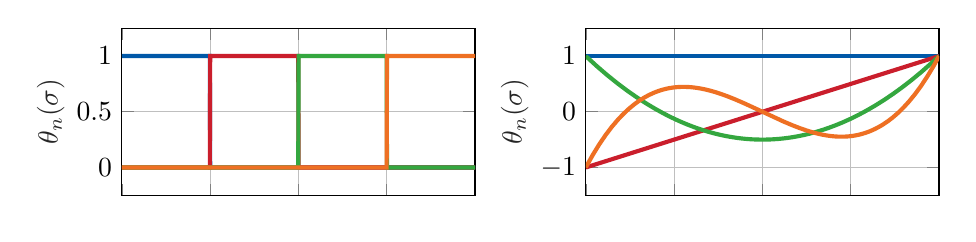
\begin{tikzpicture}

\begin{axis}[%
width=0.37\textwidth,
height=0.175\textwidth,
at={(0\textwidth,0\textwidth)},
scale only axis,
xmin=0,
xmax=1,
xtick={0,0.25,0.5,0.75,1},
xticklabels={{},{},{},{},{}},
ymin=-0.25,
ymax=1.25,
ylabel style={font=\color{white!15!black}},
ylabel={$\theta_n(\sigma)$},
axis background/.style={fill=white},
title style={font=\bfseries},
% title={$(a)$},
xmajorgrids,
ymajorgrids,
ylabel style={yshift=-2.5pt}
]
\addplot [color=mycolor1, line width=1.5pt, forget plot]
  table[row sep=crcr]{%
0	1\\
0.249249249249249	1\\
0.25025025025025	0\\
1	0\\
};
\addplot [color=mycolor2, line width=1.5pt, forget plot]
  table[row sep=crcr]{%
0	0\\
0.249249249249249	0\\
0.25025025025025	1\\
0.499499499499499	1\\
0.500500500500501	0\\
1	0\\
};
\addplot [color=mycolor3, line width=1.5pt, forget plot]
  table[row sep=crcr]{%
0	0\\
0.499499499499499	0\\
0.500500500500501	1\\
0.74974974974975	1\\
0.750750750750751	0\\
1	0\\
};
\addplot [color=mycolor4, line width=1.5pt, forget plot]
  table[row sep=crcr]{%
0	0\\
0.74974974974975	0\\
0.750750750750751	1\\
1	1\\
};
\end{axis}

\begin{axis}[%
width=0.37\textwidth,
height=0.175\textwidth,
at={(0.486\textwidth,0\textwidth)},
scale only axis,
xmin=0,
xmax=1,
xtick={0,0.25,0.5,0.75,1},
xticklabels={{},{},{},{},{}},
ymin=-1.5,
ymax=1.5,
ylabel style={font=\color{white!15!black}},
ylabel={$\theta_n(\sigma)$},
axis background/.style={fill=white},
title style={font=\bfseries},
%title={$(b)$},
xmajorgrids,
ymajorgrids,
ylabel style={yshift=-2.5pt}
]
\addplot [color=mycolor1, line width=1.5pt, forget plot]
  table[row sep=crcr]{%
0	1\\
1	1\\
};
\addplot [color=mycolor2, line width=1.5pt, forget plot]
  table[row sep=crcr]{%
0	-1\\
1	1\\
};
\addplot [color=mycolor3, line width=1.5pt, forget plot]
  table[row sep=crcr]{%
0	1\\
0.0310310310310311	0.819591363134907\\
0.0610610610610611	0.656004352701049\\
0.0900900900900901	0.508156805454103\\
0.118118118118118	0.375002630257885\\
0.145145145145145	0.255531808084361\\
0.171171171171171	0.148770392013635\\
0.196196196196196	0.0537805072339606\\
0.22022022022022	-0.0303396489582677\\
0.243243243243243	-0.10445580715851\\
0.265265265265265	-0.169397625854082\\
0.286286286286286	-0.225958691424157\\
0.307307307307307	-0.277217157097037\\
0.327327327327327	-0.321104888672456\\
0.346346346346346	-0.358343328313298\\
0.364364364364364	-0.389617846074302\\
0.381381381381381	-0.415577739902064\\
0.397397397397397	-0.436836235635034\\
0.413413413413414	-0.455016578139701\\
0.428428428428429	-0.469265060856652\\
0.442442442442442	-0.480122765408051\\
0.456456456456456	-0.488623758894029\\
0.469469469469469	-0.494407320233146\\
0.482482482482482	-0.498158819480141\\
0.495495495495496	-0.499878256635014\\
0.507507507507508	-0.499661823986148\\
0.519519519519519	-0.497713930146363\\
0.532532532532533	-0.493649805962118\\
0.545545545545546	-0.487553619685752\\
0.558558558558559	-0.479425371317263\\
0.572572572572573	-0.468399330261192\\
0.586586586586587	-0.455016578139701\\
0.601601601601602	-0.438062687311937\\
0.617617617617618	-0.416996576155735\\
0.633633633633634	-0.392852311771231\\
0.650650650650651	-0.363826288751214\\
0.668668668668669	-0.329305281257233\\
0.687687687687688	-0.288639991342694\\
0.707707707707708	-0.241145048952857\\
0.727727727727728	-0.188840492143795\\
0.748748748748749	-0.128744359975591\\
0.770770770770771	-0.0600991381772165\\
0.793793793793794	0.0178887596305013\\
0.817817817817818	0.106048991934878\\
0.842842842842843	0.205247289331373\\
0.868868868868869	0.316385454523592\\
0.894894894894895	0.435651868084301\\
0.921921921921922	0.56810864918973\\
0.94994994994995	0.714729744759775\\
0.978978978978979	0.876525173822471\\
1	1\\
};
\addplot [color=mycolor4, line width=1.5pt, forget plot]
  table[row sep=crcr]{%
0	-1\\
0.0190190190190189	-0.782485871940692\\
0.0380380380380381	-0.585849574761409\\
0.0560560560560561	-0.418072891875022\\
0.0740740740740742	-0.267591322461007\\
0.0910910910910911	-0.14071778835241\\
0.107107107107107	-0.0342981766697772\\
0.123123123123123	0.0600275897464979\\
0.138138138138138	0.137912741624562\\
0.153153153153153	0.206008053341874\\
0.167167167167167	0.26108942025359\\
0.18018018018018	0.305205863277448\\
0.193193193193193	0.342823368979655\\
0.205205205205205	0.372007618203764\\
0.216216216216216	0.394270823050955\\
0.227227227227227	0.412405233898399\\
0.237237237237237	0.425443028180901\\
0.246246246246246	0.434472266818126\\
0.255255255255255	0.441030078586554\\
0.264264264264264	0.445204206451941\\
0.272272272272272	0.446984357566612\\
0.28028028028028	0.447012056580584\\
0.288288288288288	0.445348928183114\\
0.297297297297297	0.441533571555485\\
0.306306306306306	0.435743998198344\\
0.316316316316316	0.427102419377978\\
0.327327327327327	0.41505036134801\\
0.339339339339339	0.399043011303921\\
0.352352352352352	0.378569076902044\\
0.367367367367367	0.351233983600084\\
0.383383383383384	0.318131447265587\\
0.401401401401401	0.276624908126279\\
0.422422422422422	0.223395060218871\\
0.447447447447447	0.154754895576799\\
0.481481481481481	0.0554285423969925\\
0.55955955955956	-0.174453117166602\\
0.585585585585586	-0.244218652545899\\
0.606606606606607	-0.295588205146412\\
0.625625625625626	-0.337224912399687\\
0.641641641641642	-0.368091627977139\\
0.656656656656657	-0.393078784510256\\
0.66966966966967	-0.411320689517806\\
0.681681681681682	-0.42510521776274\\
0.692692692692693	-0.434982658462395\\
0.702702702702703	-0.441533571555485\\
0.711711711711712	-0.445348928183114\\
0.720720720720721	-0.447102325115474\\
0.728728728728729	-0.446858939689107\\
0.736736736736737	-0.444855399075886\\
0.744744744744745	-0.441030078586554\\
0.753753753753754	-0.434472266818126\\
0.762762762762763	-0.425443028180901\\
0.771771771771772	-0.413854619709123\\
0.781781781781782	-0.3978703949716\\
0.792792792792793	-0.376369795653945\\
0.803803803803804	-0.350609329511154\\
0.815815815815816	-0.317460398130658\\
0.827827827827828	-0.278843238464521\\
0.840840840840841	-0.230596015489016\\
0.854854854854855	-0.170884130911225\\
0.868868868868869	-0.10280934270289\\
0.883883883883884	-0.020216582116821\\
0.898898898898899	0.0727618041999487\\
0.914914914914915	0.183843708779055\\
0.931931931931932	0.315873496183937\\
0.948948948948949	0.462912686785208\\
0.966966966966967	0.635618141204809\\
0.984984984984985	0.826515637191178\\
1	1\\
};
\end{axis}
\end{tikzpicture}%
  
    % This file was created by matlab2tikz.
%
\definecolor{mycolor1}{rgb}{0.00000,0.34510,0.65882}%
\definecolor{mycolor2}{rgb}{0.79216,0.11765,0.17255}%
\definecolor{mycolor3}{rgb}{0.20392,0.65490,0.24706}%
\definecolor{mycolor4}{rgb}{0.93333,0.43922,0.13725}%
%
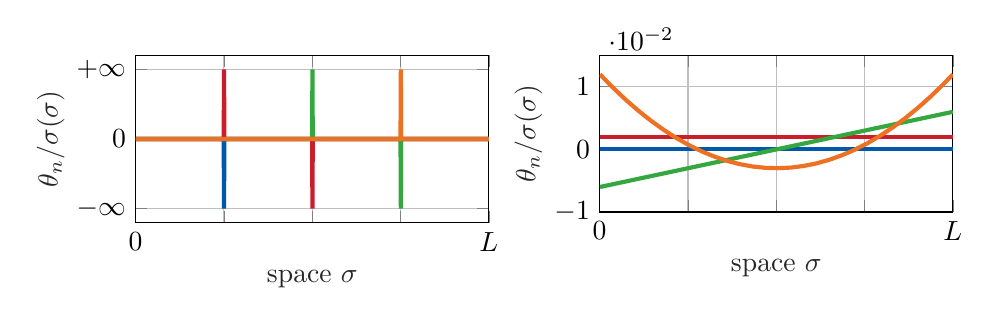
\begin{tikzpicture}

\begin{axis}[%
width=0.37\textwidth,
height=0.175\textwidth,
at={(0\textwidth,0\textwidth)},
scale only axis,
xmin=0,
xmax=1,
xtick={0,0.25,0.5,0.75,1},
xticklabels={{0},{},{},{},{$L$}},
ytick={-1,0,1},
yticklabels={{$-\infty$},0,{$+\infty$}},
xlabel style={font=\color{white!15!black}},
xlabel={space $\sigma$},
ymin=-1.2,
ymax=1.2,
ylabel style={font=\color{white!15!black}},
ylabel={$\p \theta_n/\p \sigma (\sigma)$},
axis background/.style={fill=white},
xmajorgrids,
ymajorgrids,
ylabel style={yshift=-2.5pt}
]
\addplot [color=mycolor1, line width=1.5pt, forget plot]
  table[row sep=crcr]{%
0.00100100100100109	0\\
0.249249249249249	0\\
0.25025025025025	-1\\
0.251251251251251	0\\
1	0\\
};
\addplot [color=mycolor2, line width=1.5pt, forget plot]
  table[row sep=crcr]{%
0.00100100100100109	0\\
0.249249249249249	0\\
0.25025025025025	1\\
0.251251251251251	0\\
0.499499499499499	0\\
0.500500500500501	-1\\
0.501501501501502	0\\
1	0\\
};
\addplot [color=mycolor3, line width=1.5pt, forget plot]
  table[row sep=crcr]{%
0.00100100100100109	0\\
0.499499499499499	0\\
0.500500500500501	1\\
0.501501501501502	0\\
0.74974974974975	0\\
0.750750750750751	-1\\
0.751751751751752	0\\
1	0\\
};
\addplot [color=mycolor4, line width=1.5pt, forget plot]
  table[row sep=crcr]{%
0.00100100100100109	0\\
0.74974974974975	0\\
0.750750750750751	1\\
0.751751751751752	0\\
1	0\\
};
\end{axis}

\begin{axis}[%
width=0.37\textwidth,
height=0.164\textwidth,
at={(0.486\textwidth,0.011\textwidth)},
scale only axis,
xmin=0,
xmax=1,
xtick={0,0.25,0.5,0.75,1},
xticklabels={{0},{},{},{},{$L$}},
xlabel style={font=\color{white!15!black}},
xlabel={space $\sigma$},
ymin=-0.01,
ymax=0.015,
ylabel style={font=\color{white!15!black}},
ylabel={$\p \theta_n/\p \sigma(\sigma)$},
axis background/.style={fill=white},
xmajorgrids,
ymajorgrids,
ylabel style={yshift=-2.5pt}
]
\addplot [color=mycolor1, line width=1.5pt, forget plot]
  table[row sep=crcr]{%
0.00100100100100109	0\\
1	0\\
};
\addplot [color=mycolor2, line width=1.5pt, forget plot]
  table[row sep=crcr]{%
0.00100100100100109	0.00200200200200196\\
1	0.00200200200200196\\
};
\addplot [color=mycolor3, line width=1.5pt, forget plot]
  table[row sep=crcr]{%
0.00100100100100109	-0.00599999398798179\\
1	0.00599999398798179\\
};
\addplot [color=mycolor4, line width=1.5pt, forget plot]
  table[row sep=crcr]{%
0.00100100100100109	0.0119819719820118\\
0.037037037037037	0.00989780573368138\\
0.0730730730730731	0.00796962698002934\\
0.109109109109109	0.00619743572105302\\
0.145145145145145	0.00458123195675597\\
0.181181181181181	0.00312101568713552\\
0.217217217217217	0.00181678691219256\\
0.253253253253253	0.000668545631927309\\
0.289289289289289	-0.000323708153660229\\
0.325325325325325	-0.00115997444457028\\
0.361361361361361	-0.00184025324080306\\
0.397397397397397	-0.0023645445423579\\
0.433433433433434	-0.00273284834923548\\
0.469469469469469	-0.00294516466143557\\
0.505505505505506	-0.00300149347895817\\
0.541541541541542	-0.00290183480180284\\
0.577577577577578	-0.00264618862997024\\
0.613613613613614	-0.00223455496346037\\
0.64964964964965	-0.00166693380227234\\
0.685685685685686	-0.000943325146407048\\
0.721721721721722	-6.37289958642651e-05\\
0.757757757757758	0.000971854649356008\\
0.793793793793794	0.00216342578925377\\
0.82982982982983	0.00351098442382924\\
0.865865865865866	0.00501453055308221\\
0.901901901901902	0.00667406417701244\\
0.937937937937938	0.00848958529562016\\
0.973973973973974	0.0104610939089056\\
1	0.0119819719820118\\
};
\end{axis}
\end{tikzpicture}%
    %\fi
    \vspace{-3mm}
    \caption{Example plot of the Constant-Strain parameterization in Chapter 3 $(a)$, and the new strain parameterization \eqref{eq:C3:chebyshev} using Chebyshev polynomials $(b)$. The ordering of the strain basis is as follows $\{\theta_1,...,\theta_4\} = \{\ldata{Matlab1},\ldata{Matlab2},\ldata{Matlab3},\ldata{Matlab4}\}$. Notice that the discontinuities in the PCC models induce spikes that directly violate the compatibility equation in \eqref{eq:C3:compatibility}.}
    \label{fig:C4:basis_example}
  \end{figure}
  %
\begin{equation}
\theta_n(\sigma) = \dfrac{2}{2^{n}(n-1)!} \dfrac{d^{n-1}}{d\sigma^{n-1}}\left[\left( \dfrac{2\sigma}{L}-1 \right)^2 -1 \right]^{n-1}
\label{eq:C3:chebyshev}
\end{equation}
%
\noindent with $n \in \Z/\{0\}$ the polynomial degree. A comparison between the proposed basis and previous method in Chapter 3 is shown in Figure \ref{fig:C4:basis_example}. Please note now that the inner product between elements of the set of modified Legendre functionals $\{\theta_n\}_{n = 1}^k$ satisfies $\inner{\theta_i}{\theta_j}_{\Xs} := \int_\Xs{\theta_i}{\theta_j} d\sigma = 0$ for $i \neq j$, and $1$ otherwise. An alternative option could be constructing the set of basis functions through the so-called '\textit{snapshot decomposition method}' using FEM-driven data \cite{Astrid2008,Duriez2013,Largilliere2015}.

\begin{rmk}
The idea of joint parameterization by investigating the relation between material and structural topology of the soft robot is explored in Chapter 5.
\end{rmk}

\subsection{Reduced-order curve kinematics}
Given the finite-dimensional truncation in \eqref{eq:trunc_2}, we can now find an expression for the finite-dimensional forward kinematics in terms of the generalized coordinates $\vec{q}$ and its velocities components $\dot{\vec{q}}$.

First, let us regard the configuration of the soft robot $\mat{g} \in \SE{3}$. Recall that the spatial evolution of the curve is described by $\p \mat{g}/\p\sigma = \mat{g} \vec{\xi}^\wedge$, see Eq. \eqref{eq:C3:xi}. Given the initial condition $\mat{g}(0,\cdot) = \mat{g}_0$, an approximation of the continuously deformable soft robot can be obtained by partial integration over the spatial domain:
%
\vspace{-2mm}
\begin{equation}
[\mat{g}]_k(\sigma,\vec{q}) = \mat{g}_0 \exp_{\SE{3}}\left[\int_0^\sigma [\hat{\vec{\xi}}]_k(s,\vec{q}) \; ds \right].
\end{equation}
%
The computation of the mapping $\exp_{\SE{3}}$ is given in Appendix \ref{app:C3:liegroup}. Please note that this nothing more than the reconstruction of the curve by integration of its tangent space along its spatial parameter $\sigma$. Next, lets regard the velocity kinematics $\vec{\eta}(\sigma,t)$ for any point $\sigma$ on the backbone curve. Using the differential property of the adjoint action $\mat{\ad}_{\vec{\xi}} = -\p /\p \sigma [\Ad_{g^{-1}}] \Ad_{g}$ \cite{Murray1994}, we can rewrite the continuous forward kinematics in \eqref{eq:C3:pde_kin} as
%
\begin{equation}
\frac{\p \vec{\eta}}{\p \sigma } = \frac{\p }{\p \sigma }\left(\mat{\Ad}_{\mat{g}^{-1}}\right) \mat{\Ad}_{\mat{g}} \vec{\eta} + \dot{\vec{\xi}}. \label{eq:eta_adg}
\end{equation}
%
Now, given the initial condition $\vec{\eta}(0,t) = \vec{0}_6$ and the approximations $[\vec{\xi}]_k$ and $[\mat{g}]_k$, we can find an approximation to the velocity twist $\vec{\eta}$ by partial integration over space:
%
\begin{equation}
[\vec{\eta}]_k(\sigma,\vec{q},\dot{\vec{q}}) = \Ad_{[\mat{g}]_k}\inv \int_0^\sigma \Ad_{[\mat{g}]_k} \mat{\Theta} \; ds \,\dot{\vec{q}} := [\mat{J}]_k\, \dot{\vec{q}}, \label{eq:C3:eta_analytic}
\end{equation}
%
which naturally gives rise to the geometric Jacobian $[\mat{J}]_k \in \R^{6\times 6k}$. The geometric Jacobian plays an important role in obtaining the Lagrangian form of the reduced-order dynamic model. Finally, to express the acceleration twist, we take the time-derivative of \eqref{eq:C3:eta_analytic} leading to
%
\begin{align}{}
[\dot{\vec{\eta}}]_k & = [\mat{J}]_k\ddot{\vec{q}} + \dot{[\mat{J}]}_k\dot{\vec{q}}, \notag \\
& = [\mat{J}]_k\ddot{\vec{q}} + \Ad_{[\mat{g}]_k}\inv \int_0^\sigma \Ad_{[\mat{g}]_k} \ad_{[\vec{\eta}]_k} \mat{\Theta} \; ds \,\dot{q} \label{eq:C3:deta_analytic},
\end{align}
%
which gives rise to the analytic expression of the time-derivative of the geometric Jacobian $\dot{[\mat{J}]}_k$ (see Appendix \ref{app:C3:jacobian} for the derivation).

\subsection{Reduced-order curve dynamics using Newton-Euler}
Here, we detail the dynamics of the Cosserat beam. A majority of the dynamic framework presented here is adopted from Boyer et al. (2021, \cite{Boyer2021}); yet we introduce some modification to allow a pH-structure. First, let us consider an infinitesimal slice of continuum body that is perpendicular to the backbone curve. The kinetic momenta of this infinitesimal slice is then given by $\vec{\mu}(\sigma,t) := \MT \vec{\eta}(\sigma,t)$ in which $\MT \in \cose{3} \times \seg{3} \cong \R^{6\times 6}$ denotes the symmetric inertia tensor.
%
\begin{rmk}
For some soft robots, the inertia tensor $\MT$ may have an explicit dependency on space or time (or both). Nevertheless, for sake of simplicity, we limit ourselves to a diagonal invariant inertia tensor:
%
\begin{equation*}
\MT(\sigma,t) \cong \MT = \begin{pmatrix} \rho_0 \ten{J}  & \vec{0}_{3\times3}  \\[0.35em]
  \vec{0}_{3\times3} & \rho_0\, A\mat{I}_3 \end{pmatrix} \succ 0,
\end{equation*}
%
in which the (cross-sectional average) density is $\rho_0 > 0$, the cross-sectional area of the soft robot by $A>0$, and the second moment of area $\mat{\mathcal{J}} \in \coso{3} \times \sog{3} \cong \R^{3\times 3}$.
\end{rmk}
%
\noindent Using the expression of the kinetic momenta $\muB(\sigma,t)$ of the infinitesimal rigid body in free-motion, we can write the equation of motion for a particular slice at $\sigma$ using the Newton-Euler equations:
%
\begin{equation}
\frac{\p }{\p t} (\Ad_{\gB}^{-\top} \vec{\mu}) = \Ad_{g}^{-\top}\ten{F},\label{eq:C3:newton_euler}
\end{equation}
%
where again $\Ad_{(\cdot)}$ stands for the adjoint action, and $\ten{F} = \ten{F}_c  + \ten{F}_u - \ten{F}\grav - \ten{F}\elastic$ the resultant wrench that is composed of the constraint wrench $\ten{F}_c$, the input wrench $\ten{F}_u$, and the potential wrenches due to gravity and visco-elasticity, $\ten{F}\grav$ and $\ten{F}\elastic$, respectively. Further evaluation of \eqref{eq:C3:newton_euler} leads to
%
\begin{equation}
\MT\dot{\vec{\eta}} - \ad_{\vec{\eta}}^\top \MT \vec{\eta} = \ten{F},
\label{eq:C3:newton-euler-2}
\end{equation}
%
where we used the fact that $\dot{\Ad}_{\vec{g}} \inv = -\ad_{\vec{\eta}} {\Ad}_{\vec{g} \inv}$. Before continuing, we introduce a slight modification to the relation above. Using the fact that $\ad_{\vec{\eta}} \vec{\eta} = \vec{0}_6$, we can introduce the vector
$\ten{M} \ad_{\vec{\eta}} \vec{\eta}$ to \eqref{eq:C3:newton-euler-2} without affecting the dynamics. The importance of this modification originates from the preservation of passivity in the Lagrangian model, which is an important property in stability theorems for robotics. By substitution of the null vector, the equation of motion becomes
%
\begin{equation}
  \MT \dot{\vec{\eta}} + \left(\MT \ad_{\vec{\eta}}  - \ad_{\vec{\eta}} ^\top \MT \right) \vec{\eta} = \FT,
  \label{eq:C3:newton-euler-3}
\end{equation}
%
which is nothing more than the Newton-Euler equation for rigid-body motion on $\R^3$. To introduce the (reduced-order) Cosserat kinematics and make the expression symmetric, we substitute \eqref{eq:C3:eta_analytic} and \eqref{eq:C3:deta_analytic} into \eqref{eq:C3:newton-euler-3} and pre-multiply by $[\JB]_k^\top$:
%
\begin{multline}
  [\vec{J}]_k^\top \left( \MT [\mat{J}]_k \ddot{\vec{q}} + \MT [\dJB]_k\dot{\vec{q}} + \CT_{[\vec{\eta}]_k }\dot{\vec{q}}\right) = [\mat{J}]_k^\top \left(\FT_u - \FT\grav - \FT\elastic \right),
  \label{eq:C3:projected_NE_jacobian}
\end{multline}
%
where $\CT_{(\cdot)} = -\CT_{(\cdot)} ^\top :=  \MT \ad_{(\cdot)}  - \ad_{(\cdot)} ^\top \MT$ is a skew-symmetric matrix. It is important to note that by pre-multiplication of the transpose Jacobian, we have eliminated the constraint wrenches, \ie, $[\JB]_k^\top \FT_c = \vec{0}_n$ \cite{Murray1994}. Finally, the finite-dimensional dynamics of the deformable soft robot is found by spatial integration of \eqref{eq:C3:projected_NE_jacobian} over the material domain $\Xs$. The overall dynamics can be written in familiar Euler-Lagrangian (EL) form as follows
%
\begin{equation}
  \mat{M}(\vec{q})\ddot{\vec{q}} + \mat{C}(\vec{q},\dot{\vec{q}})\dot{\vec{q}} + \vec{f}\!\grav(\vec{q}) + \vec{f}\!\elastic(\vec{q},\dot{\vec{q}}) = \vec{\tau}(\vec{q},\uB)
  \label{eq:C3:dyn_model_lag}
\end{equation}
%
with the system matrices:
%
\begin{align}
 \MB(\q) & = \int_\Xs [\mat{J}]_k^\top \ten{M} [\mat{J}]_k \; d \sigma, \label{eq:C3:lag_M} \\
 \mat{C}(\q,\dq) & = \int_\Xs [\JB]_k^\top \!\left(\ten{M} [\dJB]_k + \ten{C}_{{[\vec{\eta}]}_k}[\mat{J}]_k \right) \; d \sigma, \label{eq:C3:lag_C} \\
\vec{f}\!\grav(\q) & = \int_\Xs [\JB]_k^\top \ten{F}\!\grav \; d \sigma, \\
\vec{f}\!\elastic(\q,\dq) & = \int_\Xs [\JB]_k^\top \ten{F}\!\elastic \; d \sigma := \mat{K}\vec{q} + \mat{D}\dot{\vec{q}},
\label{eq:C3:lag_G} \\
\vec{\tau}(\q,\uB) & = \int_\Xs [\mat{J}]_k^\top \ten{F}_u \; d\sigma := \mat{G} \vec{u}, \label{eq:C3:lag_tau}
\end{align}
%
\noindent where $\mat{M}$ is the generalized inertia matrix, $\mat{C}$ the  centripetal-Coriolis matrix, $\fB\!\grav$ a vector of generalized potential forces with $\ten{F}\!\grav = -\Ad_{[\gB]_k}^\top \ten{M} \vec{a}_g$ the external wrench acting on the body due to gravitational acceleration $\vec{a}_g$, and $\ten{F}_e$ a vector of visco-elastic forces imposed by the stiffness matrix $\mat{K} \succ 0$ and damping matrix $\vec{D} \succ 0$. Following the procedures in finite elements and assuming linear visco-elasticity, the stiffness matrix and damping matrix are computed through spatial integration:
%
\begin{align}
\mat{K} = \int_\Xs \mat{\Theta}^\top \!\mat{\mathcal{K}}\, \mat{\Theta} \; d\sigma, \label{eq:C3:stiff_mat}\\
\mat{D} = \int_\Xs \mat{\Theta}^\top \!\mat{\mathcal{D}}\, \mat{\Theta} \; d\sigma, \label{eq:C3:damp_mat}
\end{align}
%
where $\mat{\mathcal{K}} \in \cose{3} \times \seg{3}$ and $\mat{\mathcal{D}} \in  \cose{3} \times \seg{3}$ are the stiffness and damping tensor, respectively. The vector $\vec{Gu}$ represents the distributed forces and torques generated by various kinds of the internal actuators (\eg, tendons or pneumatics). Again, system of matrices can then be efficiently recovered using a Matrix-Differential solver proposed in Chapter 3. If $\rank(\GB) < \dim(\q)$, a system is said to be under-actuated. Within the context of soft robotics, whose infinite-dimensional configuration space cannot be matched by a finite number of actuators, these systems are often intrinsically under-actuated. 

\begin{lem}
  \label{lem:C3:1}
  The inertia matrix $\mat{M}(\vec{q})$ is a symmetric, positive definite, symmetric. and is uniformly bounded such that there exists positive constants $\lambda^{-} \le \lambda^{+}$ such that  $\lambda^{-} \mat{I}_{n} \preceq \mat{M}(\vec{q}) \preceq \lambda^{+} \mat{I}_{n} < \infty$.
\end{lem}

\begin{proof}
Proof can be found in Spong et al. (2006, \citep{Spong2006}).
\end{proof}

\begin{lem}
\label{lem:C3:passive}
Given the inertia matrix $\mat{M}(\vec{q})$ and the Coriolis matrix
$\mat{C}(\vec{q},\dot{\vec{q}})$ as described by \eqref{eq:C3:lag_M} and \eqref{eq:C3:lag_C}, respectively, it can be shown that the matrix $\dot{\mat{M}} - 2\mat{C}$ is skew-symmetric.
\end{lem}

\begin{proof}
To show $\dot{\mat{M}} - 2\mat{C}$ is skew-symmetric, we start by computing the time-derivative of the inertia matrix. For sake of clarity, lets abbreviate the Jacobians matrices $[\mat{J}]_k = \mat{J}$ and $[\dJB]_k = \dJB$. Through chain differentiation, we find
%
\begin{equation}
\dot{\mat{M}} = \int_\Xs \dJB^\top \ten{M} \mat{J} + \mat{J}^\top \ten{M} \dJB\; d \sigma,
\end{equation}
%
Then, calculating $\dot{\mat{M}} - 2\mat{C}$ leads to
%
\begin{align}
\dot{\mat{M}} - 2\mat{C} & = \int_\Xs \dJB^\top \ten{M} \mat{J} - \mat{J}^\top \ten{M} \dJB - 2\mat{J}^\top \!\ten{C} \, \mat{J} \; d\sigma.
\end{align}
%
Since the matrix $\mat{J}^\top \ten{C} \mat{J}$ is skew-symmetric, the remainder of the proof is to show that the matrix $\mat{S} = \dJB^\top \ten{M} \mat{J} - \mat{J}^\top \ten{M} \dJB$ also satisfies skew-symmetry. Since the inertia tensor is symmetric $\ten{M} = \ten{M}^\top
$, we can easily show this holds true:
%
\begin{align}
\mat{S} & = \dJB^\top \MT^\top \mat{J} - \mat{J}^\top \MT^\top \dJB, \notag \\
 & = -\left(\dJB^\top \ten{M}^\top \mat{J} - \mat{J}^\top \ten{M} \dJB \right)^\top = -\mat{S}^\top.
\end{align}
%
Therefore, the matrix $\dot{\mat{M}(\vec{q})} - 2\mat{C}(\vec{q},\dot{\vec{q}})$ is skew-symmetric for all $\vec{q},\dot{\vec{q}} \in \R^n$
\end{proof}

In literature, Lemma \ref{lem:C3:passive} is often referred to as the passivity condition \cite{Spong2006,Ortega1998,Murray1994}. It implies that, in the absence of external dissipation, the total energy of the system (\ie, the Hamiltonian) is conserved. It is also worth mentioning that this condition does not necessarily hold true for all cases, only for particular computations of the Coriolis matrix $\mat{C}(\vec{q},\vec{\dot{q}})$ (\eg, through the Christoffel symbols).

\subsection{Port-Hamiltonian formulation}
In this section, the Lagrangian model in \eqref{eq:C3:dyn_model_lag} is rewritten in port-Hamiltonian form. To this end, we define the generalized momenta $\vec{p} := \mat{M} \dot{\vec{q}}$. Then, the (reduced-order) Hamiltonian is given by
$\mathcal{H}(\vec{q},\vec{p}) := \Kf(\vec{q},\vec{p}) + \Uf(\vec{q})$ with $\Kf = \frac{1}{2} \vec{p}^\top \mat{M}\inv \vec{p}$ and $\Uf(\vec{q})$ the kinetic and potential energy, respectively.

Given the system's Hamiltonian $\mathcal{H}$, it can be shown that generalized velocities can be written in terms of partial derivatives of the Hamiltonian function
%
\begin{equation}
\dot{\vec{q}} = \nabla_{\vec{p}} \Hm \quad \Longrightarrow  \quad \nabla_{\vec{p}} \Hm := \left(\frac{\p \Hm}{\p \pB} \right)^\top= \mat{M}\inv \vec{p}.
\label{eq:C3:state_diff}
\end{equation}
%
where we denote $\nabla_{\xB}(\cdot) := \p (\cdot)^\top/\p \xB$ as the gradient w.r.t. a vector field $\xB$. Note that $\mat{M}^{-1}$ is always exists due to the positive definiteness condition in Lemma \ref{lem:C3:1}. Similarly, we seek a differential description that relates the time evolution of $\vec{p}$ to a state-derivative of the Hamiltonian function. Applying the chain rule of differentiation to the generalized momenta:
%
\begin{align}
\dot{\vec{p}} & = \dot{\mat{M}}\dot{\vec{q}} + \mat{M}\ddot{\vec{q}},\notag \\
& = \left(\dot{\mat{M}} - \mat{C} - \mat{D} \right) \mat{M}\inv \vec{p} - \vec{Kq} - \vec{f}\!\grav + \vec{Gu}
\label{eq:C3:momenta_diff1},
\end{align}
%
Taking the partial derivative of the Hamiltonian $\Hm$ w.r.t. the generalized coordinates $\vec{q}$, we find
 %
\begin{align}
\nabla_{\vec{q}} \Hm & = \frac{1}{2} \,\nabla_{\!\q} \left[ \dot{\vec{q}}^\top \mat{M}(\vec{q}) \dot{\vec{q}} \right] + \nabla_{\!\vec{q}}\, \mathcal{U}.
\label{eq:C3:ham_momenta_diff}
\end{align}
%
To relate \eqref{eq:C3:momenta_diff1} and \eqref{eq:C3:ham_momenta_diff}, we explores some structural properties in the Lagrangian model. To be more specific, we exploit the skew-symmetry condition as detailed in Lemma \ref{lem:C3:passive}. According to the Spong et al. (2006, \cite{Spong2006}), if the matrix $\dot{\mat{M}} - 2\mat{C}$ satisfies the passivity condition in Lemma \ref{lem:C3:passive}, it can be shown that
%
\begin{equation}
\left( \dot{\mat{M}} - 2\mat{C} \right) \dot{\vec{q}} =  -\nabla_{\vec{q}} \left[ \dot{\vec{q}}^\top \mat{M}(\vec{q}) \dot{\vec{q}} \right] - \dot{\mat{M}}\dot{\vec{q}}. \label{eq:C3:skew_mat_equal}
\end{equation}
%
Finally, by combining \eqref{eq:C3:state_diff}, \eqref{eq:C3:momenta_diff1}, \eqref{eq:C3:ham_momenta_diff}, and \eqref{eq:C3:skew_mat_equal}, we can show that the Lagrangian model in \eqref{eq:C3:dyn_model_lag} can be equivalently rewritten as a standard port-Hamiltonian (pH) system:
\begin{align}
\Sigma_{\textrm{beam}}: 
\begin{cases}
\dot{\vec{q}} \;=\; \nabla_{\vec{p}} \Hm, \\[0.25em]
\dot{\vec{p}} \;=\; -\nabla_{\vec{q}} \Hm - \mat{D}\nabla_{\vec{p}} \Hm + \vec{Gu}.
\end{cases}
\label{eq:C3:model_ph}
\end{align}
%
The advantage of the port-Hamiltonian system $\Sigma_\textrm{beam}$ over the standard EL structure in \eqref{eq:C3:dyn_model_lag}, and as also seen in Chapter 3, is the general applicability to different physical domains and the common formalism with energy-based control, which we will explore further in the next section. By collocating the state variable into a state vector $\x = (\q^\top, \pB^\top)^\top$, we may write the system into an equivalent form: $\dx = \left(\JT - \RT \right)\grad{\x}\!\Hm(\x) + \BT(\x)\uB$, where $\JT = -\JT^\top$ a skew-symmetric matrix, $\RT \succeq 0$ a positive semi-definite dissipation matrix. 